\documentclass[12pt]{beamer}\usepackage[]{graphicx}\usepackage[]{color}
%% maxwidth is the original width if it is less than linewidth
%% otherwise use linewidth (to make sure the graphics do not exceed the margin)
\makeatletter
\def\maxwidth{ %
  \ifdim\Gin@nat@width>\linewidth
    \linewidth
  \else
    \Gin@nat@width
  \fi
}
\makeatother

\definecolor{fgcolor}{rgb}{0.345, 0.345, 0.345}
\newcommand{\hlnum}[1]{\textcolor[rgb]{0.686,0.059,0.569}{#1}}%
\newcommand{\hlstr}[1]{\textcolor[rgb]{0.192,0.494,0.8}{#1}}%
\newcommand{\hlcom}[1]{\textcolor[rgb]{0.678,0.584,0.686}{\textit{#1}}}%
\newcommand{\hlopt}[1]{\textcolor[rgb]{0,0,0}{#1}}%
\newcommand{\hlstd}[1]{\textcolor[rgb]{0.345,0.345,0.345}{#1}}%
\newcommand{\hlkwa}[1]{\textcolor[rgb]{0.161,0.373,0.58}{\textbf{#1}}}%
\newcommand{\hlkwb}[1]{\textcolor[rgb]{0.69,0.353,0.396}{#1}}%
\newcommand{\hlkwc}[1]{\textcolor[rgb]{0.333,0.667,0.333}{#1}}%
\newcommand{\hlkwd}[1]{\textcolor[rgb]{0.737,0.353,0.396}{\textbf{#1}}}%
\let\hlipl\hlkwb

\usepackage{framed}
\makeatletter
\newenvironment{kframe}{%
 \def\at@end@of@kframe{}%
 \ifinner\ifhmode%
  \def\at@end@of@kframe{\end{minipage}}%
  \begin{minipage}{\columnwidth}%
 \fi\fi%
 \def\FrameCommand##1{\hskip\@totalleftmargin \hskip-\fboxsep
 \colorbox{shadecolor}{##1}\hskip-\fboxsep
     % There is no \\@totalrightmargin, so:
     \hskip-\linewidth \hskip-\@totalleftmargin \hskip\columnwidth}%
 \MakeFramed {\advance\hsize-\width
   \@totalleftmargin\z@ \linewidth\hsize
   \@setminipage}}%
 {\par\unskip\endMakeFramed%
 \at@end@of@kframe}
\makeatother

\definecolor{shadecolor}{rgb}{.97, .97, .97}
\definecolor{messagecolor}{rgb}{0, 0, 0}
\definecolor{warningcolor}{rgb}{1, 0, 1}
\definecolor{errorcolor}{rgb}{1, 0, 0}
\newenvironment{knitrout}{}{} % an empty environment to be redefined in TeX

\usepackage{alltt}
\usepackage{tikz}

% make it pretty
% get rid of junk
\usetheme{default}
\usefonttheme[onlymath]{serif}
\beamertemplatenavigationsymbolsempty

% define a bunch of colors
\definecolor{offwhite}{RGB}{255,250,240}
\definecolor{gray}{RGB}{155,155,155}
\definecolor{foreground}{RGB}{80,80,80}
\definecolor{background}{RGB}{255,255,255}
%\definecolor{title}{RGB}{255,199,0}
\definecolor{title}{RGB}{89,132,212}
%\definecolor{subtitle}{RGB}{89,132,212}
\definecolor{subtitle}{RGB}{255,199,0}
\definecolor{hilit}{RGB}{248,117,79}
\definecolor{vhilit}{RGB}{255,111,207}
\definecolor{lolit}{RGB}{200,200,200}
\definecolor{lit}{RGB}{255,199,0}
\definecolor{mdlit}{RGB}{89,132,212}
\definecolor{link}{RGB}{248,117,79}

% a few color macros
\newcommand{\hilit}{\color{hilit}}
\newcommand{\vhilit}{\color{vhilit}}
\newcommand{\lit}{\color{lit}}
\newcommand{\mdlit}{\color{mdlit}}
\newcommand{\lolit}{\color{lolit}}

% use those colors
\setbeamercolor{titlelike}{fg=title}
\setbeamercolor{subtitle}{fg=subtitle}
\setbeamercolor{frametitle}{fg=gray}
%\setbeamercolor{structure}{fg=subtitle}
\setbeamercolor{structure}{fg=title}
\setbeamercolor{institute}{fg=lolit}
\setbeamercolor{normal text}{fg=foreground,bg=background}
\setbeamertemplate{itemize subitem}{{\textendash}}
\setbeamerfont{itemize/enumerate subbody}{size=\small}
\setbeamerfont{itemize/enumerate subitem}{size=\small}

% center title of slides
\setbeamertemplate{blocks}[rounded]
\setbeamertemplate{frametitle}[default][center]

% page number
\setbeamerfont{page number in foot}{size=\footnotesize}
\setbeamertemplate{footline}[frame number]

% default link color
\hypersetup{colorlinks, urlcolor={link}}

% a few macros
\newcommand{\code}[1]{\texttt{#1}}
\newcommand{\hicode}[1]{{\hilit \texttt{#1}}}
\newcommand{\locode}[1]{{\lolit \texttt{#1}}}
\newcommand{\bb}[1]{\begin{block}{#1}}
\newcommand{\eb}{\end{block}}
\newcommand{\bi}{\begin{itemize}}
\newcommand{\bbi}{\vspace{4pt} \begin{itemize} \itemsep8pt}
\newcommand{\ei}{\end{itemize}}
\newcommand{\bv}{\begin{verbatim}}
\newcommand{\ev}{\end{verbatim}}
\newcommand{\ig}{\includegraphics}
\newcommand{\subt}[1]{{\footnotesize \color{subtitle} {#1}}}
\newcommand{\ttsm}{\tt \small}
\newcommand{\ttfn}{\tt \footnotesize}
\newcommand{\figh}[2]{\centerline{\includegraphics[height=#2\textheight]{#1}}}
\newcommand{\figw}[2]{\centerline{\includegraphics[width=#2\textwidth]{#1}}}



%------------------------------------------------

\title{Inertia: Multivariate Dispersion}
\subtitle{Matrix Algebra 4 Statistical Learning}
\author{\href{http://www.gastonsanchez.com}{Gaston Sanchez}}
\institute{\href{https://creativecommons.org/licenses/by-sa/4.0/}{\tt \scriptsize \color{foreground} CC BY-SA 4.0}}
\date{}
\IfFileExists{upquote.sty}{\usepackage{upquote}}{}
\begin{document}



% no page number in first slide
{
  \setbeamertemplate{footline}{} 
  \frame{\titlepage} 
}

%------------------------------------------------

\begin{frame}
\begin{center}
\Huge{\hilit{Introduction}}
\end{center}
\end{frame}

%------------------------------------------------

\begin{frame}
\frametitle{NBA Team Stats}

\bbi
  \item NBA Team Stats: regular season (2016-17)
  \item Github file: \code{data/nba-teams-2017.csv}
  \item Source: \textbf{stats.nba.com}
  \item \url{http://stats.nba.com/teams/traditional/\#!?sort=GP\&dir=-1}
\ei

\end{frame}

%------------------------------------------------

{ % image occupying entire slide.
    \begin{frame}[plain]
        \begin{tikzpicture}[remember picture,overlay]
            \node[at=(current page.center)] {
                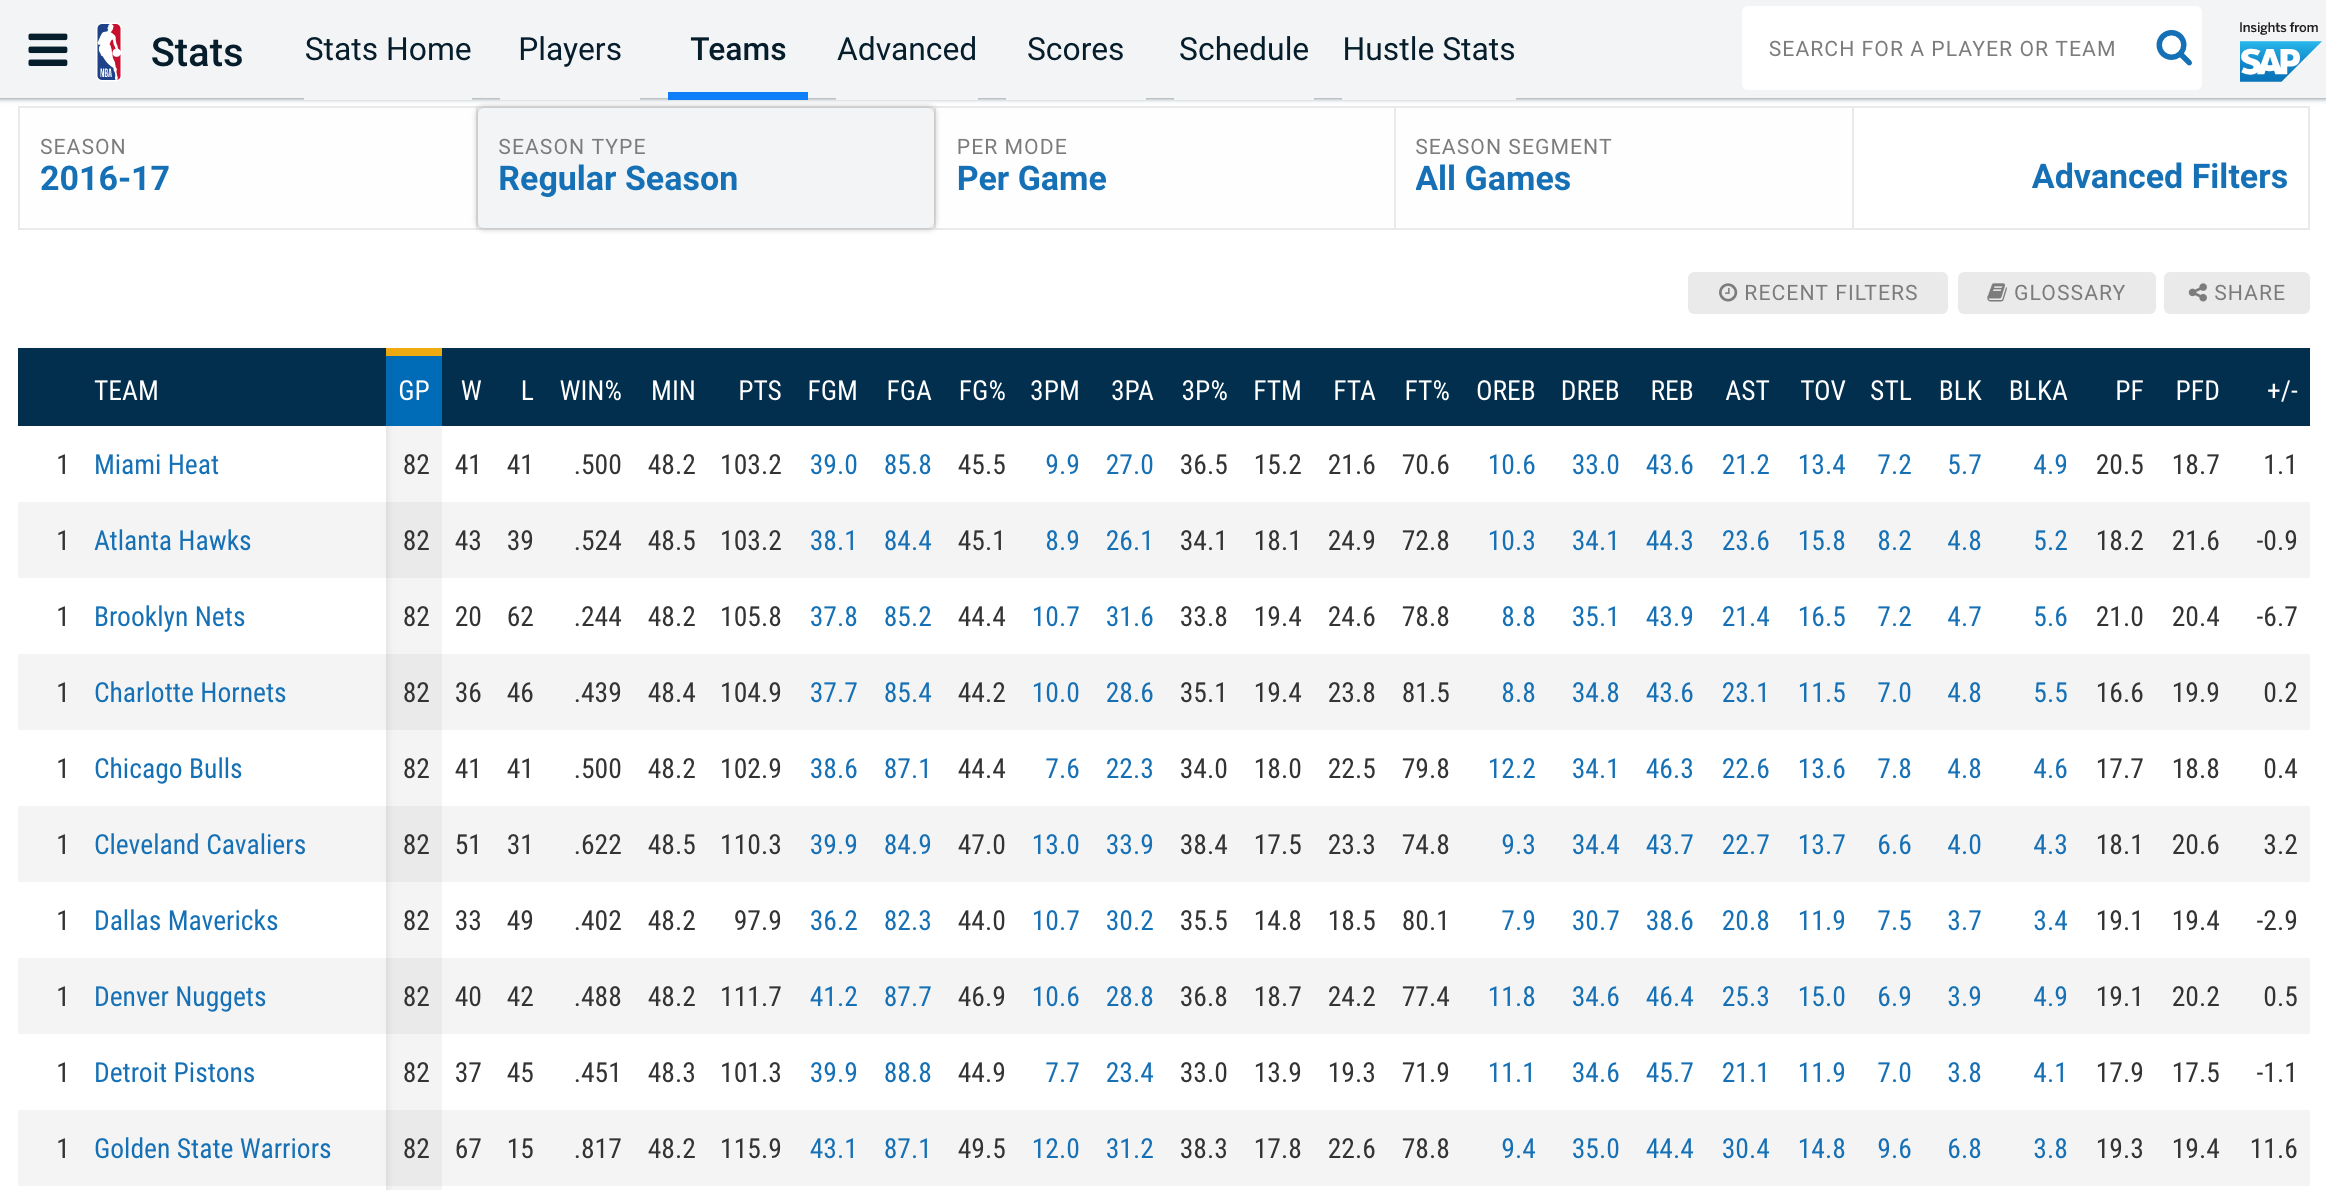
\includegraphics[width=\paperwidth]{images/nba-stats-2017.png}
            };
        \end{tikzpicture}
     \end{frame}
}

%------------------------------------------------

\begin{frame}[fragile]

\begin{knitrout}\scriptsize
\definecolor{shadecolor}{rgb}{0.969, 0.969, 0.969}\color{fgcolor}\begin{kframe}
\begin{alltt}
\hlcom{# variables}
\hlstd{dat} \hlkwb{<-} \hlkwd{read.csv}\hlstd{(}\hlstr{'data/nba-teams-2017.csv'}\hlstd{)}
\end{alltt}
\end{kframe}
\end{knitrout}



\begin{knitrout}\scriptsize
\definecolor{shadecolor}{rgb}{0.969, 0.969, 0.969}\color{fgcolor}\begin{kframe}
\begin{alltt}
\hlkwd{dim}\hlstd{(dat)}
\end{alltt}
\begin{verbatim}
[1] 30 27
\end{verbatim}
\begin{alltt}
\hlkwd{names}\hlstd{(dat)}
\end{alltt}
\begin{verbatim}
 [1] "team"                  "games_played"          "wins"                 
 [4] "losses"                "win_prop"              "minutes"              
 [7] "points"                "field_goals"           "field_goals_attempted"
[10] "field_goals_prop"      "points3"               "points3_attempted"    
[13] "points3_prop"          "free_throws"           "free_throws_att"      
[16] "free_throws_prop"      "off_rebounds"          "def_rebounds"         
[19] "rebounds"              "assists"               "turnovers"            
[22] "steals"                "blocks"                "block_fga"            
[25] "personal_fouls"        "personal_fouls_drawn"  "plus_minus"           
\end{verbatim}
\end{kframe}
\end{knitrout}

\end{frame}

%------------------------------------------------

\begin{frame}
\frametitle{Exploratory Data Analysis}

For illustration purposes, let's focus on the following variables:
\bi
  \item \code{wins}
  \item \code{losses}
  \item \code{points}
  \item \code{field\_goals}
  \item \code{assists}
  \item \code{turnovers}
  \item \code{steals}
  \item \code{blocks}
\ei

\end{frame}

%------------------------------------------------

\begin{frame}
\frametitle{EDA: Objects and Variables Perspectives}
\begin{center}
\ig[width=9cm]{images/pca_data_perspectives.pdf}
\end{center}
\end{frame}

%------------------------------------------------

\begin{frame}
\frametitle{EDA: Objects and Variables Perspectives}

\begin{block}{Data Perspectives}
We are interested in analyzing a data set from both perspectives: 
\textbf{objects} and \textbf{variables}
\end{block}

At its simplest we are interested in 2 fundamental purposes:
\bi
  \item Study resemblance among individuals \\
  {\lolit (resemblance among NBA teams)} 
  \item Study relationship among variables \\
  {\lolit (relationship among team statistics)}
\ei

\end{frame}

%------------------------------------------------

\begin{frame}
\frametitle{EDA}

\bb{Exploration}
Likewise, we can explore variables at different stages:
\bbi
  \item Univariate: one variable at a time
  \item Bivariate: two variables simultaneously
  \item Multivariate: multiple variables
\ei
\eb

Let's see a shiny-app demo (see \code{apps/} folder in github repo)

\end{frame}

%------------------------------------------------

\begin{frame}[fragile]

\begin{knitrout}\footnotesize
\definecolor{shadecolor}{rgb}{0.969, 0.969, 0.969}\color{fgcolor}

{\centering 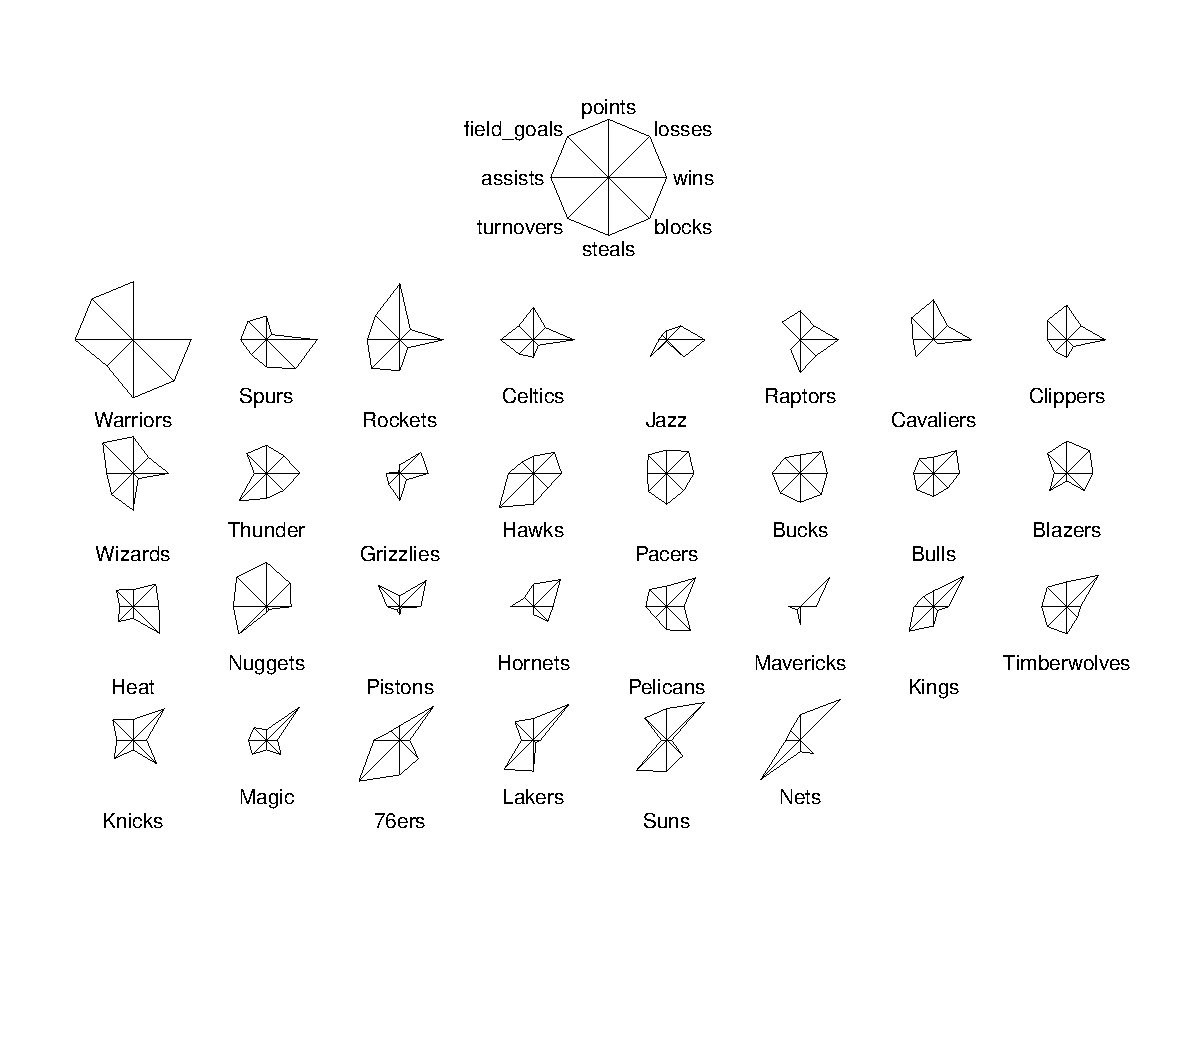
\includegraphics[width=.95\linewidth,height=.9\linewidth]{figure/stars-1} 

}



\end{knitrout}

\end{frame}

%------------------------------------------------

\begin{frame}[fragile]
\frametitle{Correlation heatmap}

\begin{knitrout}\footnotesize
\definecolor{shadecolor}{rgb}{0.969, 0.969, 0.969}\color{fgcolor}

{\centering 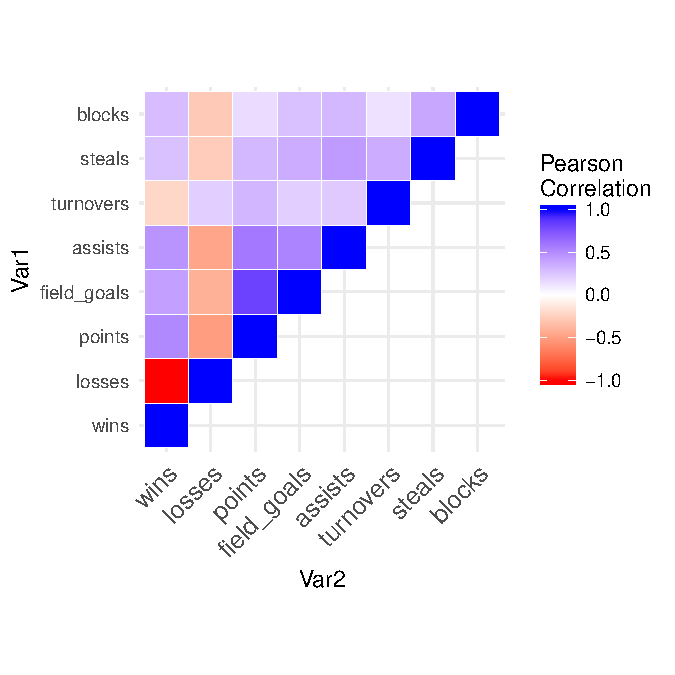
\includegraphics[width=.9\linewidth,height=.9\linewidth]{figure/cormat-1} 

}



\end{knitrout}

\end{frame}

%------------------------------------------------

\begin{frame}[fragile]

\begin{knitrout}\footnotesize
\definecolor{shadecolor}{rgb}{0.969, 0.969, 0.969}\color{fgcolor}

{\centering 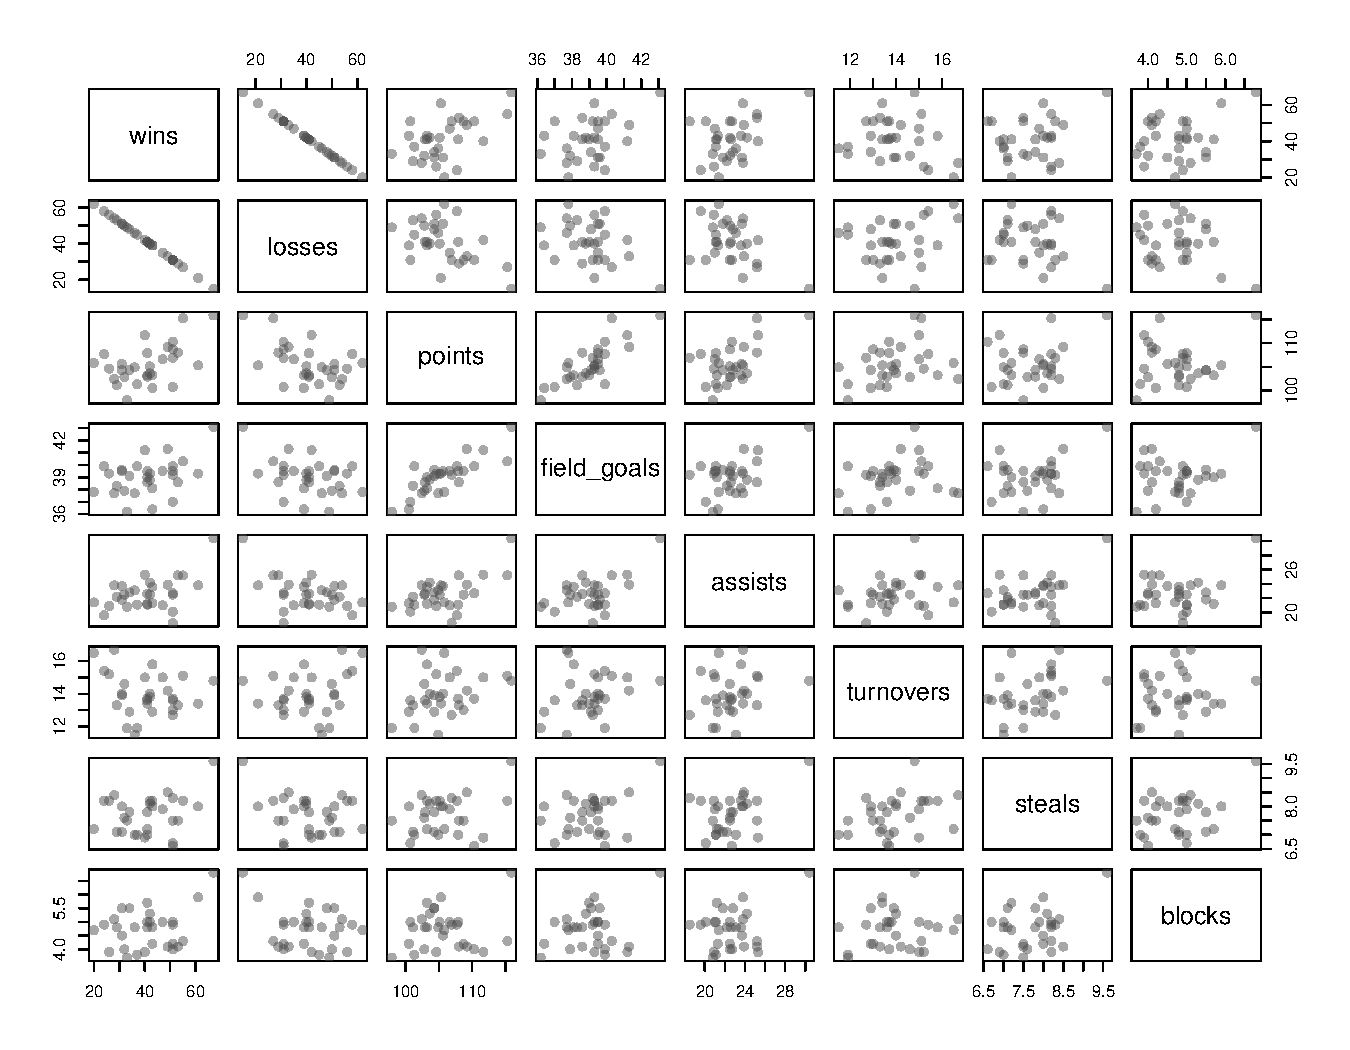
\includegraphics[width=\maxwidth]{figure/pairs-1} 

}



\end{knitrout}

\end{frame}

%------------------------------------------------

\begin{frame}
\frametitle{}

{\Large
\begin{quotation}
\noindent {\mdlit Can we get a measure of multivariate dispersion?}
\end{quotation}
}
\end{frame}

%------------------------------------------------

\begin{frame}
\begin{center}
\Huge{\hilit{How to measure dispersion? \\ 
The concept of Inertia}}
\end{center}
\end{frame}

%------------------------------------------------

\begin{frame}
\frametitle{Sum of Squared Distances}

\begin{block}{Pair-wise Squared distances}
One way to consider the dispersion of data (in a mathematical form) is by adding the 
squared distances among all pairs of points.
\end{block}

\begin{block}{Squared distances from centroid}
Another way to measure the dispersion of data is by considering the
squared distances of all points around the center of gravity (i.e. centroid)
\end{block}

\end{frame}

%------------------------------------------------

\begin{frame}
\frametitle{Imagine 3 points and its centroid}
\begin{center}
\ig[width=7cm]{images/pca_geo_square_dist1.pdf}

Centroid $\mathbf{g}$ is the ``average'' team.
\end{center}
\end{frame}

%------------------------------------------------

\begin{frame}
\frametitle{Dispersion: Sum of all squared dists}
\begin{center}
\ig[width=7cm]{images/pca_geo_square_dist2.pdf}

{\footnotesize
$\text{SSD} = 2 d^2(\text{LAL}, \text{GSW}) + 2 d^2(\text{LAL}, \text{UTA}) + 2 d^2(\text{GSW}, \text{UTA})$
}
\end{center}
\end{frame}

%------------------------------------------------

\begin{frame}
\frametitle{2n $\times$ (sum of squared dists w.r.t. centroid)}
\begin{center}
\ig[width=7cm]{images/pca_geo_square_dist3.pdf}

{\footnotesize
$\text{SSD} = (2 \times 3) \times \{ d^2(\text{LAL}, \mathbf{g}) + d^2(\text{GSW}, \mathbf{g}) + d^2(\text{UTA}, \mathbf{g}) \}$
}
\end{center}
\end{frame}

%------------------------------------------------

\begin{frame}
\frametitle{Inertia}

One way to take into account the dispersion of the data is with the concept of 
{\hilit \textbf{Inertia}}.

\bbi
  \item Inertia is a term borrowed from the \textit{moment of inertia} in mechanics (physics).
  \item This involves thinking about data as a rigid body (i.e. particles).
  \item We use the term Inertia to convey the idea of dispersion in the data.
  \item In multivariate methods, the term \textbf{\hilit Inertia generalizes the notion of variance}.
  \item Think of Inertia as a ``multidimensional variance''
\ei

\end{frame}

%------------------------------------------------

\begin{frame}
\frametitle{Cloud of teams in p-dimensional space}
\begin{center}
\ig[height=7cm]{images/pca_cloud_inertia0.pdf}
\end{center}
\end{frame}

%------------------------------------------------

\begin{frame}
\frametitle{Centroid (i.e. the average team)}
\begin{center}
\ig[height=7cm]{images/pca_cloud_inertia1.pdf}
\end{center}
\end{frame}

%------------------------------------------------

\begin{frame}
\frametitle{Formula of Total Inertia}

The Total Inertia, $I$, is a weighted sum of squared distances among all pairs of objects:
$$
I = \frac{1}{2n^2} \sum_{i = 1}^{n}{\sum_{h = 1}^{n}{d^2(i,h)}}
$$

\end{frame}

%------------------------------------------------

\begin{frame}
\frametitle{Overall variation/spread (around centroid)}
\begin{center}
\ig[height=7cm]{images/pca_cloud_inertia2.pdf}
\end{center}
\end{frame}

%------------------------------------------------

\begin{frame}
\frametitle{Formula of Total Inertia}

Equivalently, the Total Inertia can be calculated in terms of the centoid $\mathbf{g}$:
$$
I = \frac{1}{n} \sum_{i = 1}^{n}{d^2(\mathbf{x_i}, \mathbf{g})}
$$

The Inertia is an average sum of squared distances around the centroid $\mathbf{g}$

\end{frame}

%------------------------------------------------

\begin{frame}
\frametitle{Centered data: centroid is the origin}
\begin{center}
\ig[height=7cm]{images/pca_cloud_inertia3.pdf}
\end{center}
\end{frame}

%------------------------------------------------

\begin{frame}
\frametitle{Computing Inertia}

\begin{align*}
Inertia &= \sum_{i=1}^{n} m_i d^2(\mathbf{x_i}, \mathbf{g}) \\
& = \sum_{i=1}^{n} \frac{1}{n} (\mathbf{x_i} - \mathbf{g})^{\mathsf{T}}(\mathbf{x_i} - \mathbf{g}) \\
& = \frac{1}{n} tr(\mathbf{X^\mathsf{T} X}) \\
& = \frac{1}{n} tr(\mathbf{X X^\mathsf{T}})
\end{align*}

where $m_i$ is the mass (i.e. weight) of individual $i$, usually $1/n$

\end{frame}

%------------------------------------------------

\begin{frame}
\frametitle{Inertia? What for?}

\begin{block}{What's Important?}
Two data sets can have the same inertia. The amount of dispersion is important, but it is also important the shape-form of that dispersion.
\end{block}

\end{frame}

%------------------------------------------------

\begin{frame}[fragile]
\frametitle{Two data sets with similar inertia but different shape}



\begin{knitrout}\footnotesize
\definecolor{shadecolor}{rgb}{0.969, 0.969, 0.969}\color{fgcolor}

{\centering 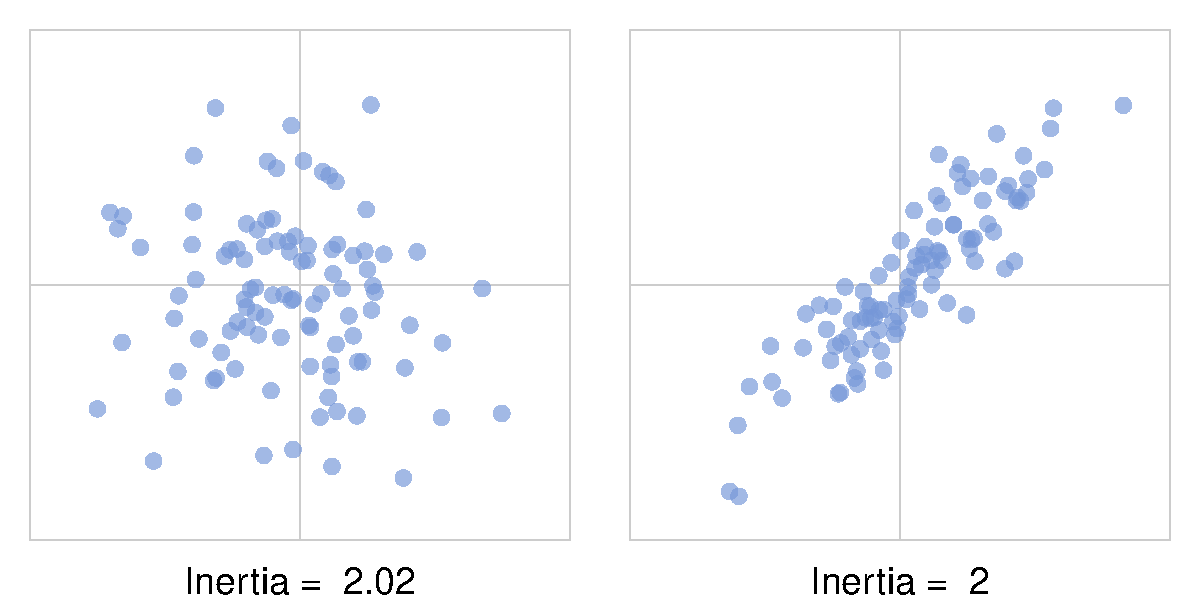
\includegraphics[width=1\linewidth,height=.5\linewidth]{figure/inertia_clouds-1} 

}



\end{knitrout}

\end{frame}

%------------------------------------------------

\end{document}
